\documentclass[11pt]{article}

\usepackage{graphicx}
\usepackage{svg}
\usepackage{amsmath}
\usepackage{amssymb}
\usepackage{mathtools}
\usepackage{pgfplots}
\usepackage{float}

\usepackage{enumerate}

\oddsidemargin=-.3in
\evensidemargin=-.5in
\textwidth=7in
\topmargin=-1in
\textheight=9.7in

\parindent=.3in
\pagestyle{plain}

\allowdisplaybreaks

\newenvironment{problems}


\begin{document}



\begin{centering}
{\huge \bf Exercise 2} \smallskip

{\Large \em Pattern Recognition, Fall 2021

Nico Aebischer

Max Jappert

}
\end{centering}

\begin{enumerate}[1.]
	\item The error rates for the three images can be seen in the output of our program, which is listed on this page. Thereafter the three outputted images are shown.
	
	\begin{verbatim}
##########-##########-##########
TRAINING DATA
(128000,)
(128000,)
----- ----- -----
Total Error WITHOUT Prior = 4894
false positive rate = 0.02415625
false negative rate = 0.014078125
----- ----- -----
Total Error WITH Prior = 4303
false positive rate = 0.0160546875
false negative rate = 0.0175625
----- ----- -----
TEST DATA PORTRAIT
(166400,)
(166400,)
----- ----- -----
Total Error WITHOUT Prior = 18044
false positive rate = 0.10468149038461538
false negative rate = 0.0037560096153846155
----- ----- -----
Total Error WITH Prior = 22715
false positive rate = 0.1323016826923077
false negative rate = 0.004206730769230769
----- ----- -----
TEST DATA FAMILY
(540000,)
(540000,)
----- ----- -----
Total Error WITHOUT Prior = 35481
false positive rate = 0.004629629629629629
false negative rate = 0.06107592592592593
----- ----- -----
Total Error WITH Prior = 43539
false positive rate = 0.003174074074074074
false negative rate = 0.0774537037037037
----- ----- -----
##########-##########-##########

	\end{verbatim}
	
	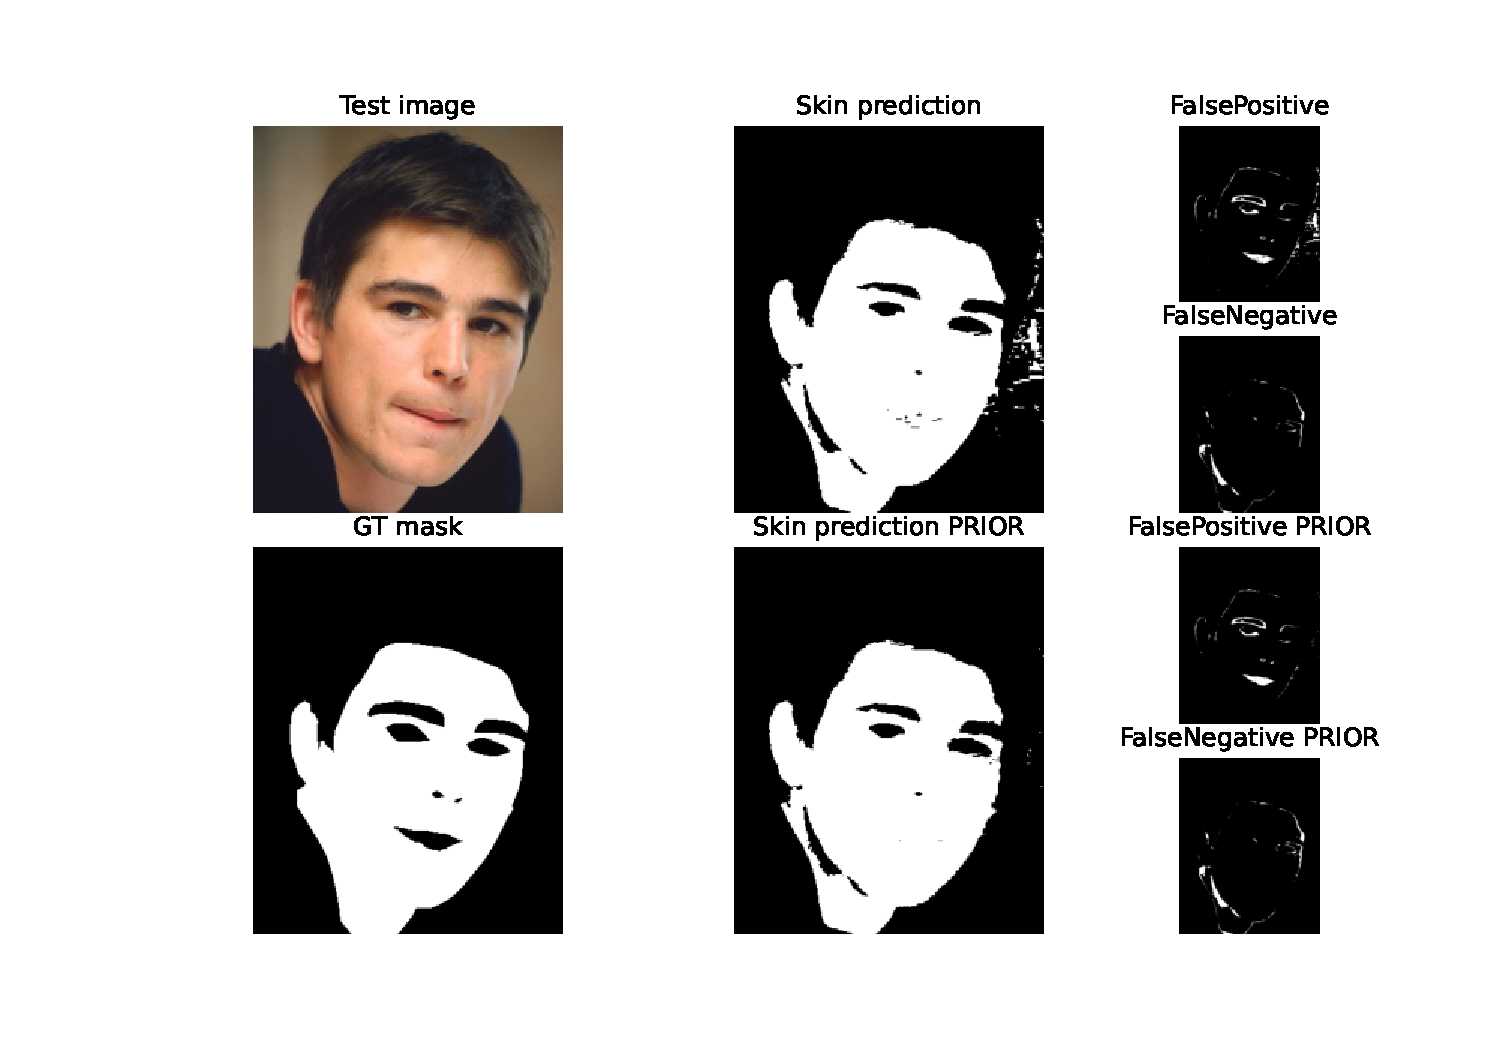
\includegraphics[width=6in]{Training-MVND.pdf}\\
	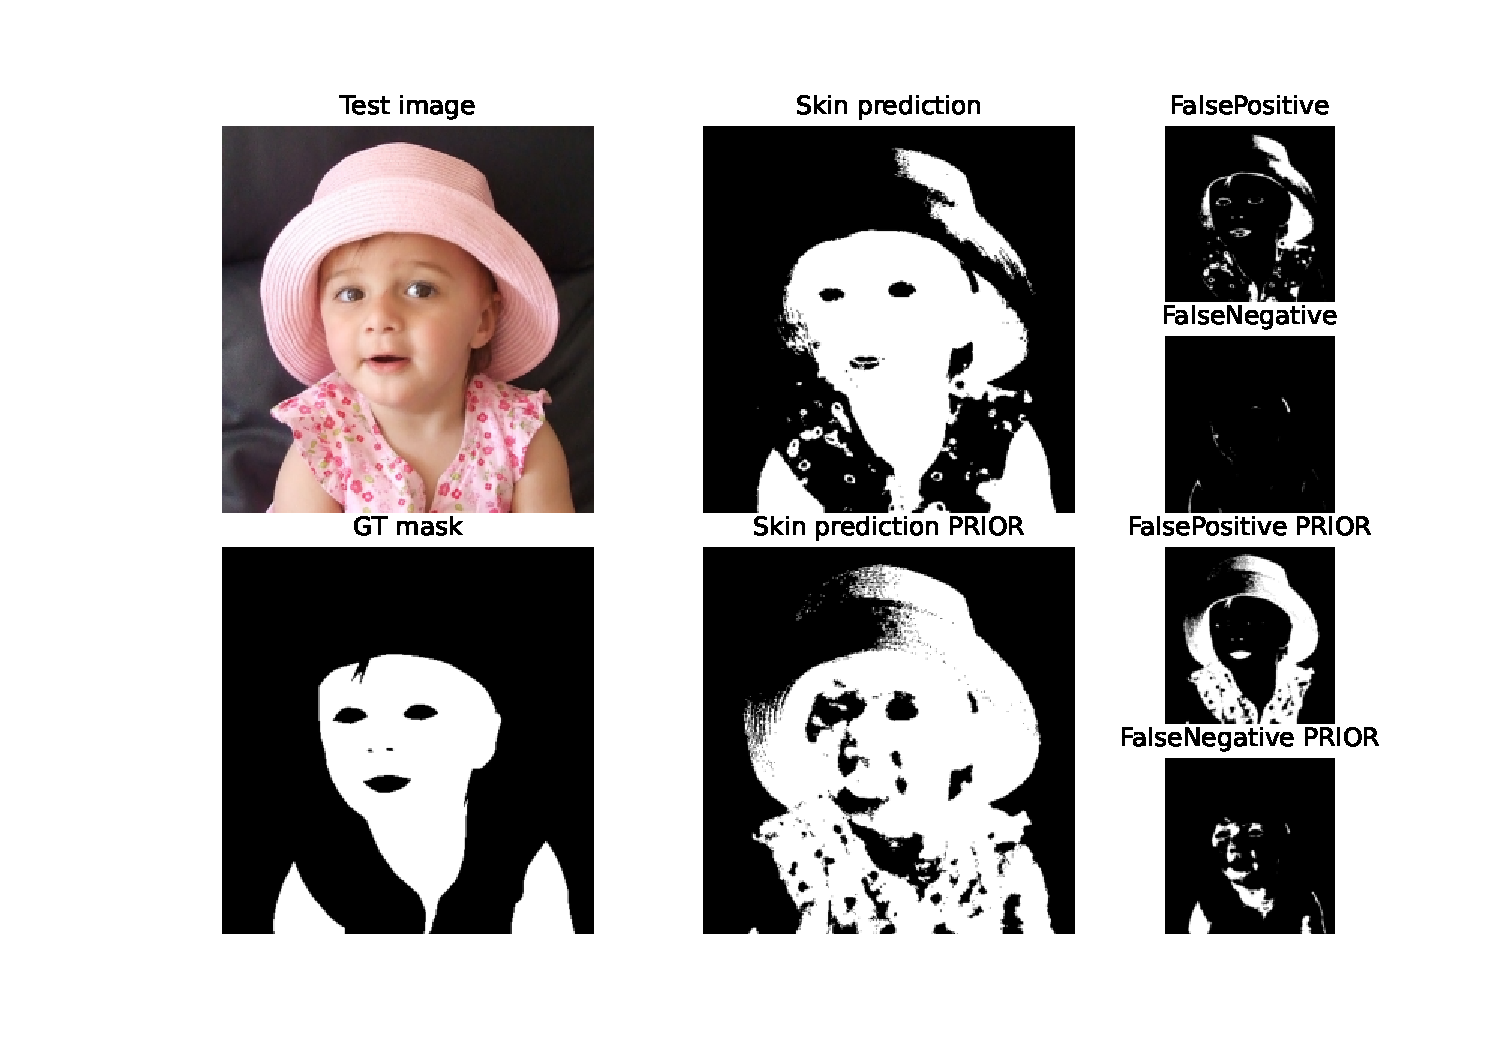
\includegraphics[width=6in]{Test-portrait-MVND.pdf}\\
	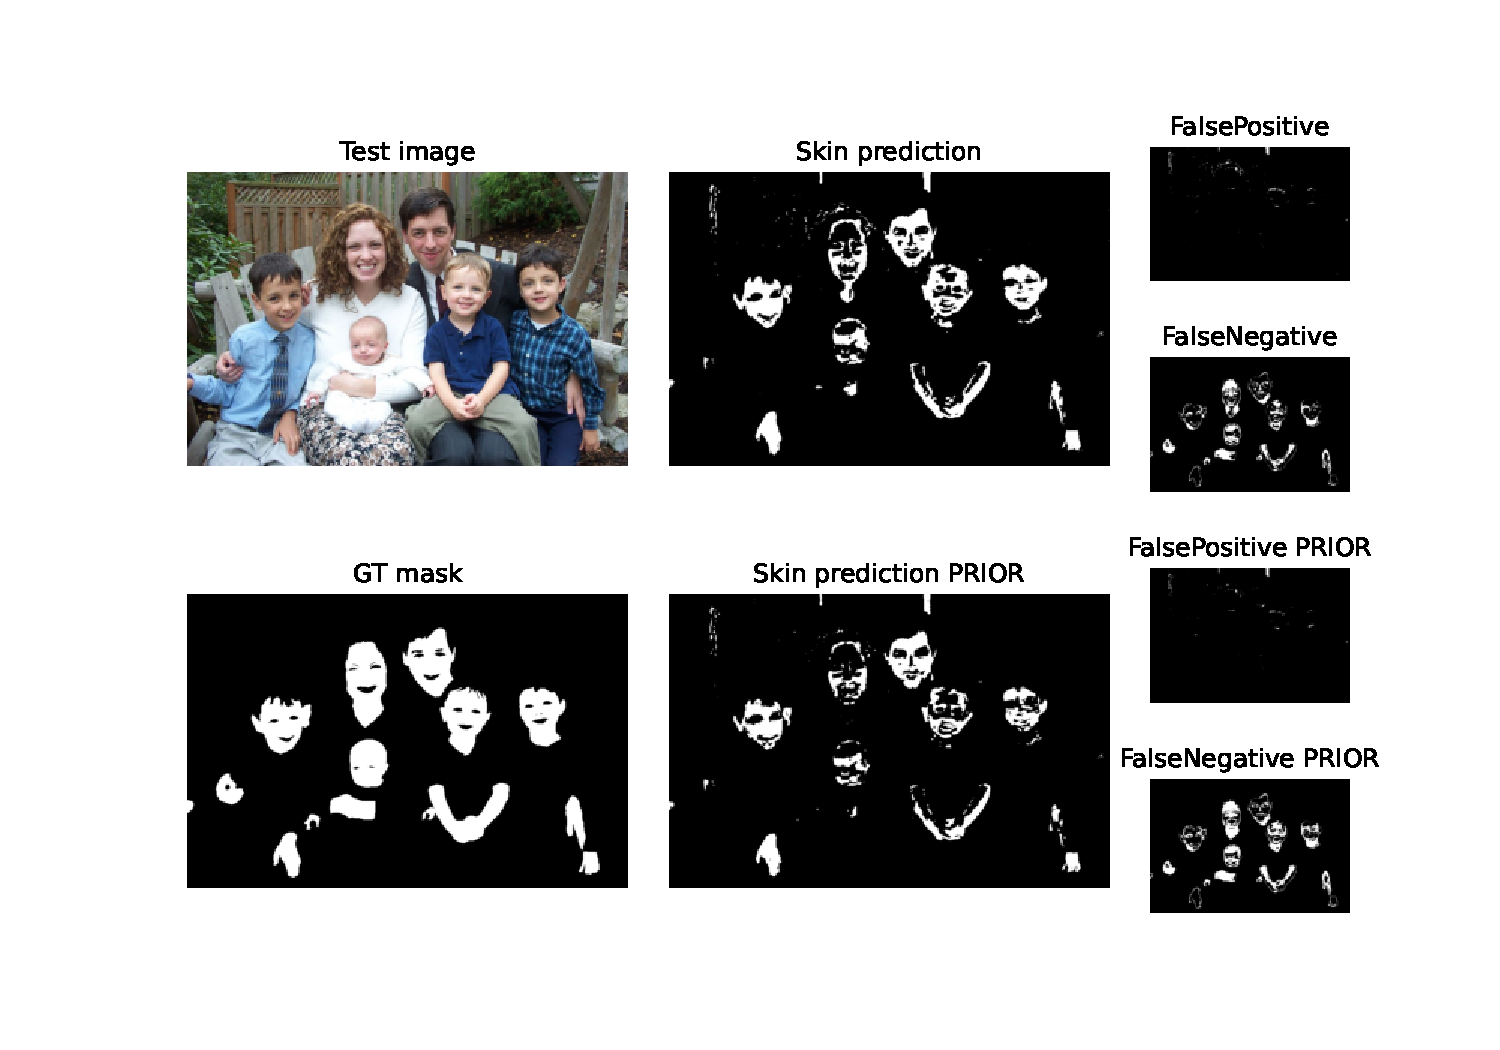
\includegraphics[width=6in]{Test-family-MVND.pdf}

	\item Skin prior: 0.3699921875\\Non-skin prior: 0.6300078124999999
	\item The prior represents the probability of a sample (in this case a pixel) belonging to a class without taking any evidence into account (in this case without considering the actual image). Therefore we calculated the priors by calculating the the proportion of the training mask which is classified as skin or non-skin for the training image. Thereby the priors represent the naive probability of a pixel belonging to each class, without considering the actual pixel to be classified. 
	\item While including the prior into the calculation improves the classification performance on the training image, the classification is less accurate with the prior included for both images the algorithm hasn't seen yet. This is because the prior has overfitted the training data. The proportion of skin in an image is not correlated to how skin can be classified generally while that proportion is very closely correlated to the image which was used for calculating this value.
	\item The results were more or less accurate, but due to the fact that the prior was created specifically for a type of picture. We therefore have to assume that it would be worse for random different types of pictures, e. g. pictures of only an arm or of a person wearing a mask. One could also estimate prior values for different types of pictures. These could be group pictures, such as portraits of individuals, landscapes with some people in it etc. Then, for each type, one could estimate the class in advance.
	\item These are the obtained cluster means from the toy example:
	\begin{enumerate}[Cluster 1:]
		\item \texttt{[-2.92220404  4.05499623]}
		\item \texttt{[5.18098269 0.89707749]}
		\item \texttt{[-2.85406695 -0.84148645]}
	\end{enumerate}
	\item This is the first figure from the toy example:
	
		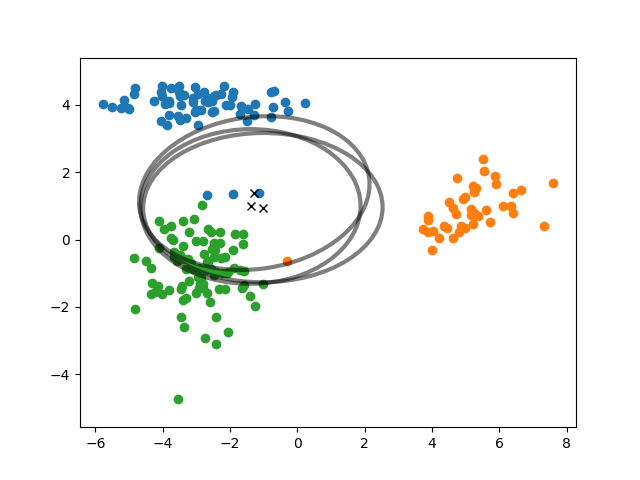
\includegraphics[width=6in]{toy_beginning.png}\\
		
		This is the final figure from the toy example:
		
		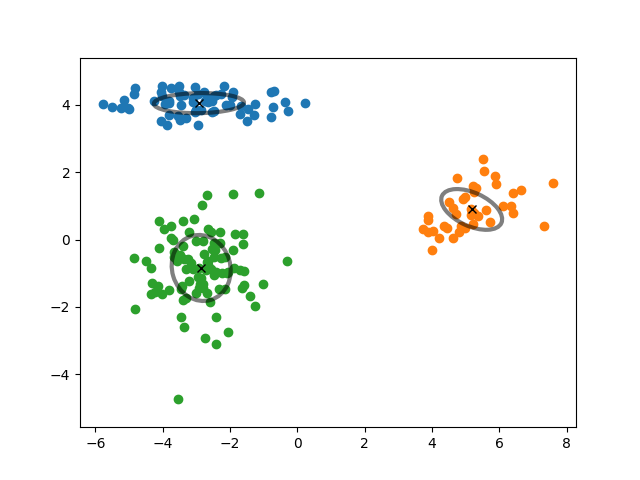
\includegraphics[width=6in]{toy_end.png}\\
	\item In this application, the variables $k$ are the hidden variables. They act as a mapping of data points to the component $k$.
	\item We had to initialize the algorithm with $\theta$. $\theta$ is made up of three components: The $c$-value, the mean vector and the covariance matrix for each class $k$. The value of $\theta$ is critical for the algorithm, because it determines the number of iterations necessary to obtain a good enough classification. If the data points (which are randomly assigned to the labels $k$ in the beginning) happen to be close to the expected classification, the algorithm terminates quite quickly while in a "bad" first assignment of points $x$ to $k$, many iterations are needed in order to come up with a good solution.
	\item No, it can converge to a local optimum which isn't the global optimum.
	\item The following is the console output for the GMM skin detection. It includes the error percentages both with and without the prior. \\
	\begin{verbatim}
GMM exercise - Skin detection
##########-##########-##########
TRAINING DATA
(128000,)
(128000,)
----- ----- -----
Total Error WITHOUT Prior = 5248
false positive rate = 0.027796875
false negative rate = 0.013203125
----- ----- -----
Total Error WITH Prior = 4393
false positive rate = 0.0214453125
false negative rate = 0.012875
----- ----- -----
skin prior:  0.3699921875
nonskin prior:  0.6300078124999999
TEST DATA PORTRAIT
(166400,)
(166400,)
----- ----- -----
Total Error WITHOUT Prior = 20252
false positive rate = 0.11887620192307692
false negative rate = 0.0028305288461538463
----- ----- -----
Total Error WITH Prior = 28862
false positive rate = 0.17165865384615384
false negative rate = 0.0017908653846153847
----- ----- -----
skin prior:  0.3699921875
nonskin prior:  0.6300078124999999
TEST DATA FAMILY
(540000,)
(540000,)
----- ----- -----
Total Error WITHOUT Prior = 33852
false positive rate = 0.005120370370370371
false negative rate = 0.05756851851851852
----- ----- -----
Total Error WITH Prior = 34285
false positive rate = 0.005520370370370371
false negative rate = 0.057970370370370373
----- ----- -----
skin prior:  0.3699921875
nonskin prior:  0.6300078124999999
##########-##########-##########

	\end{verbatim}

The next three images are the three final images which result from the GMM skin detection.\\

	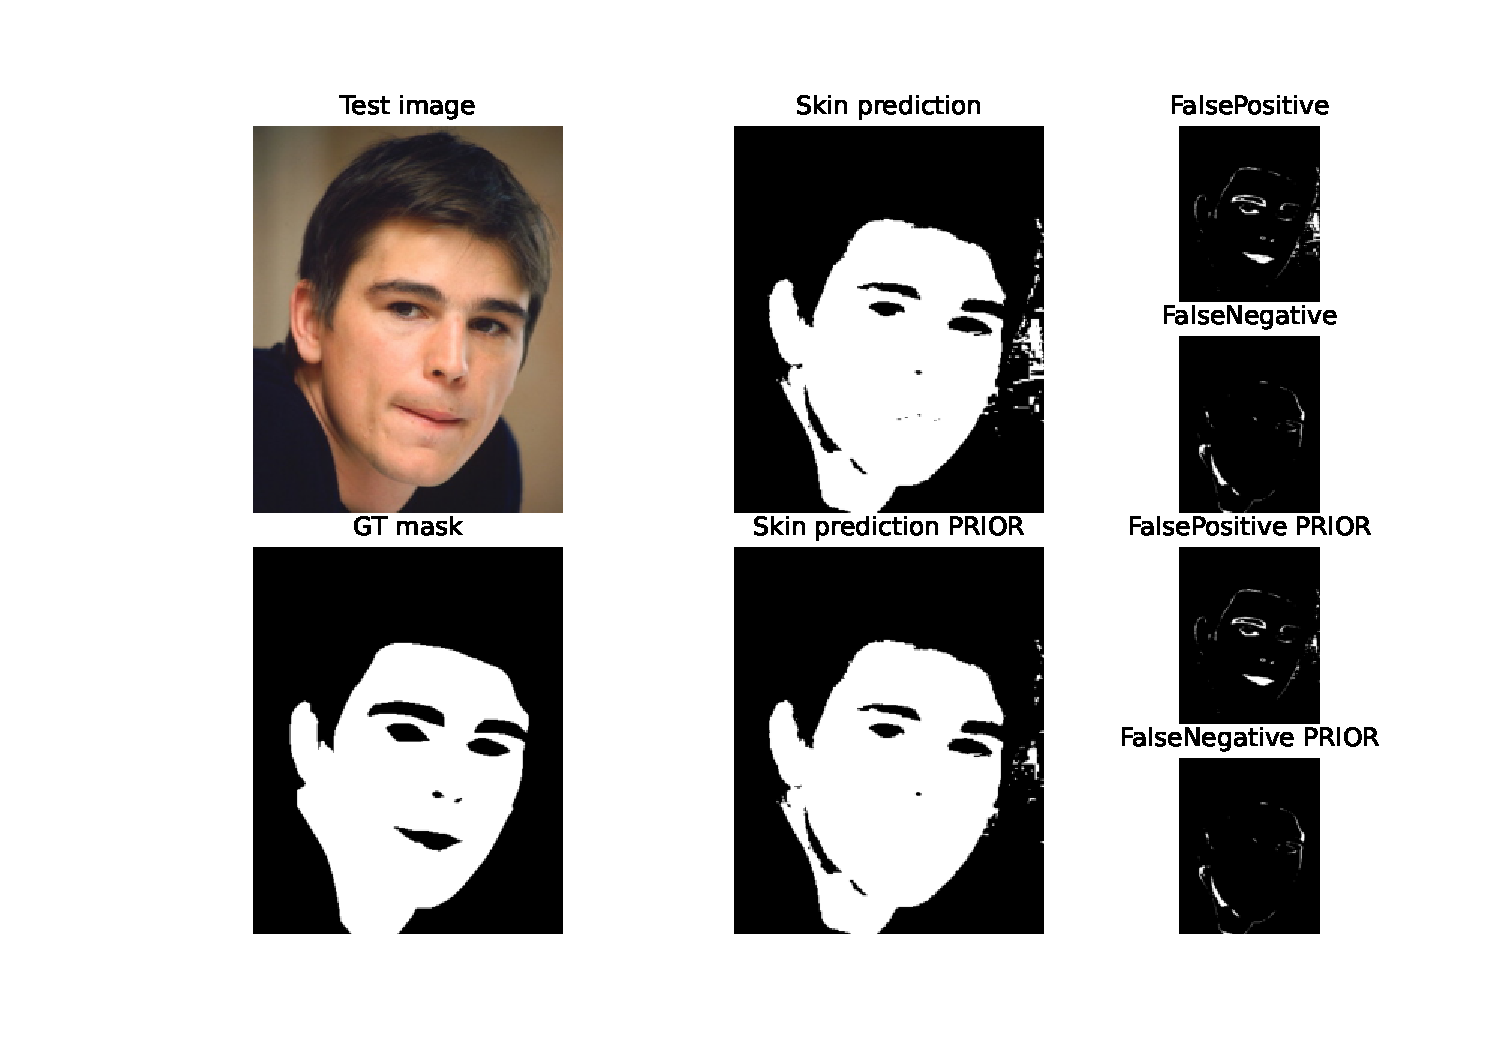
\includegraphics[width=6in]{Training-GMM.pdf}\\
	
	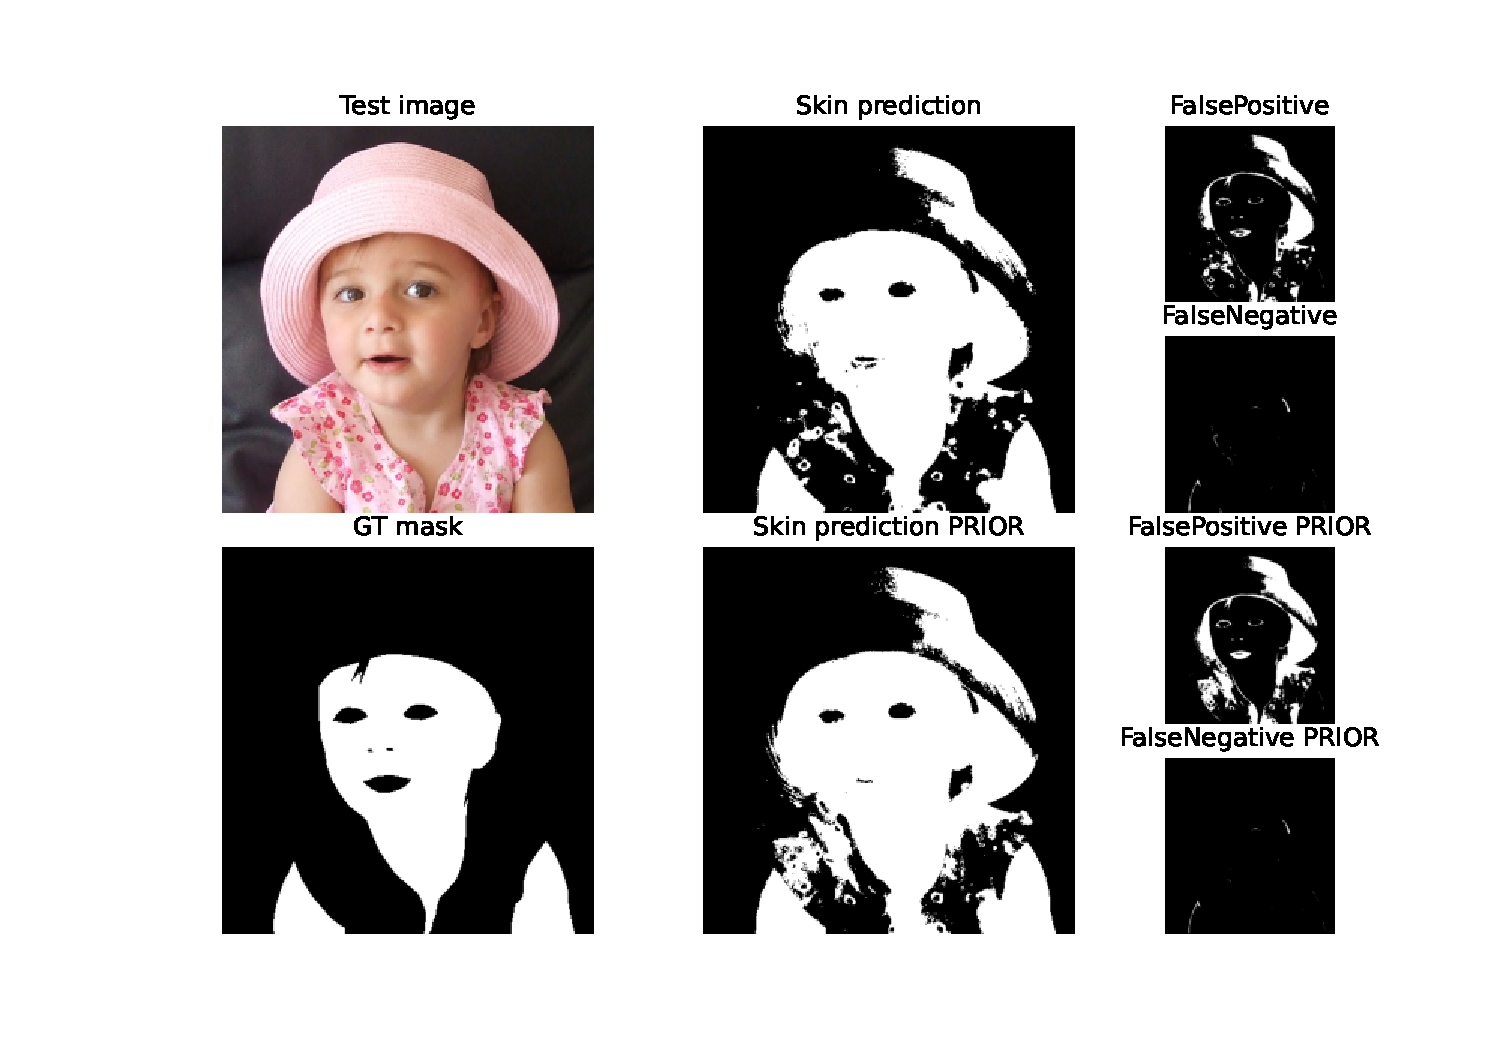
\includegraphics[width=6in]{Test-portrait-GMM.pdf}\\

	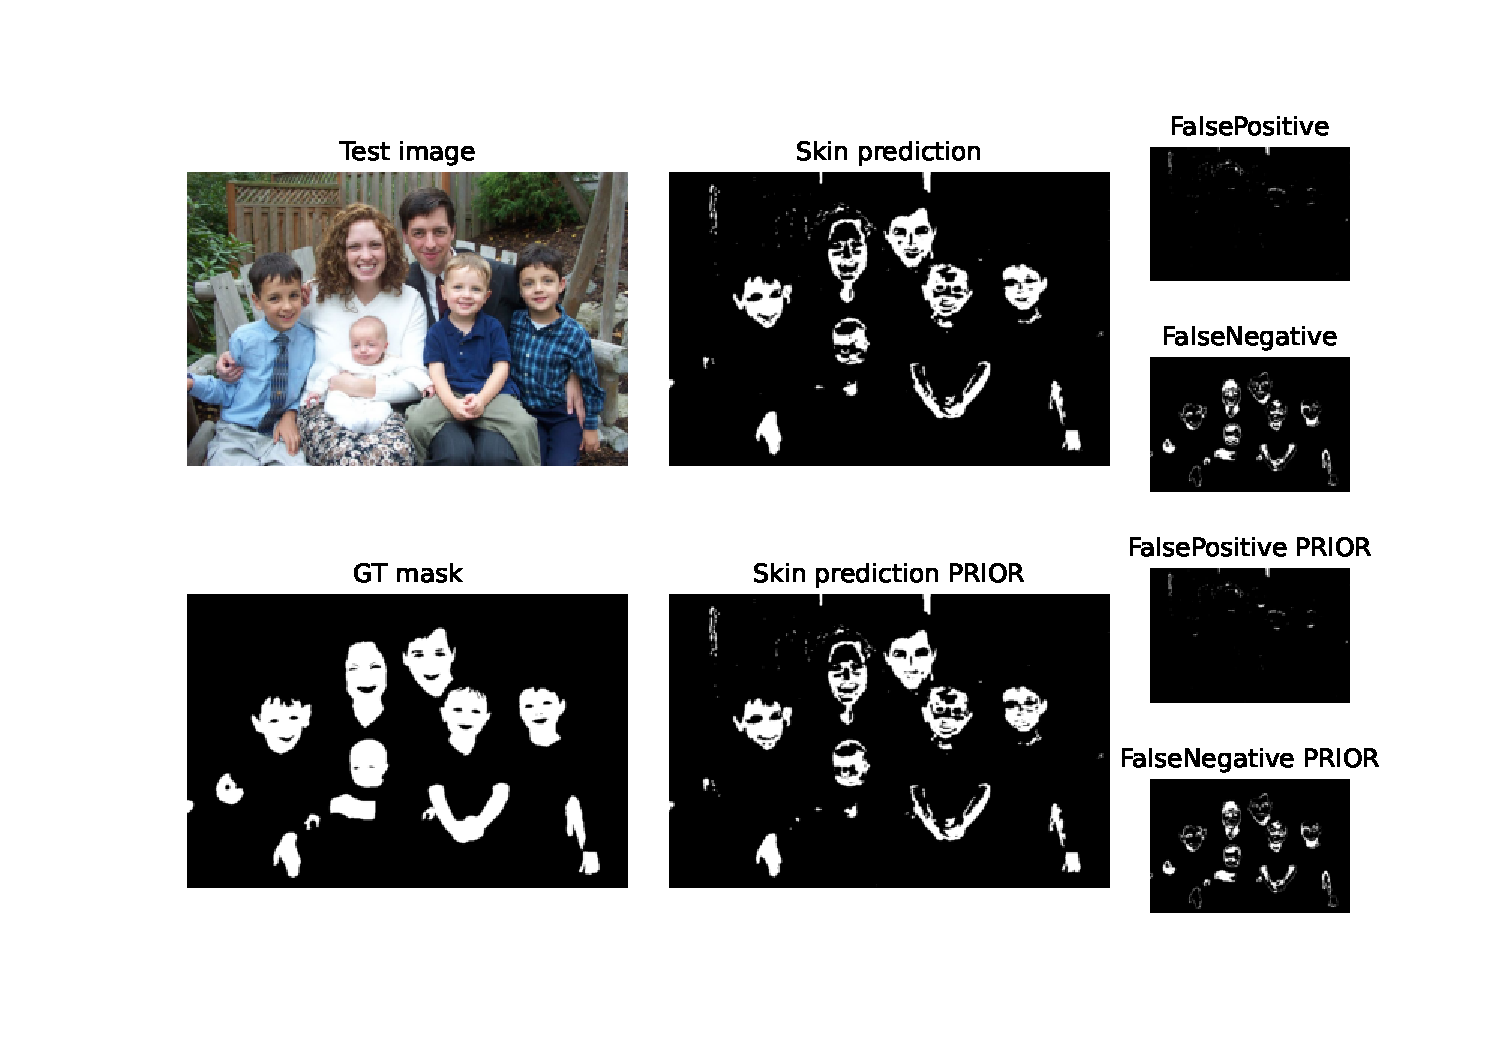
\includegraphics[width=6in]{Test-family-GMM.pdf}\\

\item The ML-principle is used to initialize an MVND. The mean and covariance are estimated according to the ML-principle.
\item In ML estimations, we do not incorporate any information about the distribution of $\theta$, except the type of distribution (e.g. normal distribution). We then estimate $\theta$ by trying to maximize the pdf for the data points. In MAP, we do not look at $\theta$ as a parameter, but as a random vector. We then use Bayes rule to find out the probability of $\theta$, using information about the distribution of it in form of the prior.
\end{enumerate}

\end{document}